% UTF-8。保留原文文字、颜色、字号、缩进和空段落；最后一项参数是可编辑文本。

% 原文段落 151；4 实现与测试
\begin{WordParagraph}{center}{18}{\WordAutoLine{18}{1.25}}{0}{0}{0}{7.8}{7.8}
\WordAutoSpaceOn
\WordRun{Times}{Hei}{18}{1}{0}{000000}{0}{4}%
\WordRun{Hei}{Hei}{18}{1}{0}{000000}{0}{\WordSpace{1}}%
\WordRun{Times}{Hei}{18}{1}{0}{000000}{0}{实现与测试}
\end{WordParagraph}

% 原文段落 152；（黑体小2加粗居中,字母、阿拉伯数字为Time New Roman小2号加粗）
\begin{WordParagraph}{center}{12}{\WordAutoLine{12}{1.25}}{0}{0}{0}{7.8}{7.8}
\WordAutoSpaceOn
\WordRun{Kai}{Kai}{12}{0}{0}{FF0000}{0}{（黑体小2加粗居中}%
\WordRun{Kai}{Kai}{12}{0}{0}{FF0000}{0}{,字母、阿拉伯数字为Time\WordSpace{1}New\WordSpace{1}Roman小2号加粗}%
\WordRun{Kai}{Kai}{12}{0}{0}{FF0000}{0}{）}
\end{WordParagraph}

% 原文段落 153；4.1实现环境与代码管理（黑体4号加粗,字母、阿拉伯数字为Time New Roman4号加粗）
\begin{WordParagraph}{both}{14}{\WordAutoLine{14}{1.25}}{0}{0}{0}{7.8}{7.8}
\WordAutoSpaceOn
\WordRun{Times}{Song}{14}{1}{0}{000000}{0}{4.1}%
\WordRun{Hei}{Hei}{14}{1}{0}{000000}{0}{实现环境与代码管理}%
\WordRun{Kai}{Kai}{12}{0}{0}{FF0000}{0}{（黑体4号加粗,字母、阿拉伯数字为Time\WordSpace{1}New\WordSpace{1}Roman4号加粗）}
\end{WordParagraph}

% 原文段落 154；这部分可首先叙述所设计软件实现的软硬件环境，代码版本管理的签入记录需截图进行说明。例如使用码云平台签入记录截图如图4-1所示（也可使用其他工具）：
\begin{WordParagraph}{both}{12}{22.5}{0}{0}{24}{0}{0}
\WordAutoSpaceOff
\WordRun{Song}{Song}{12}{0}{0}{000000}{0}{这部分可首先叙述所设计软件实现的软硬件环境，代码版本管理的签入记录需截图进行说明。例如使用码云平台签入记录截图如图}%
\WordRun{Times}{Song}{12}{0}{0}{000000}{0}{4-1}%
\WordRun{Song}{Song}{12}{0}{0}{000000}{0}{所示（也可使用其他工具）：}
\end{WordParagraph}

% 原文段落 155；
\begin{WordParagraph}{both}{12}{\WordAutoLine{12}{1}}{0}{0}{24}{0}{0}
\WordAutoSpaceOff
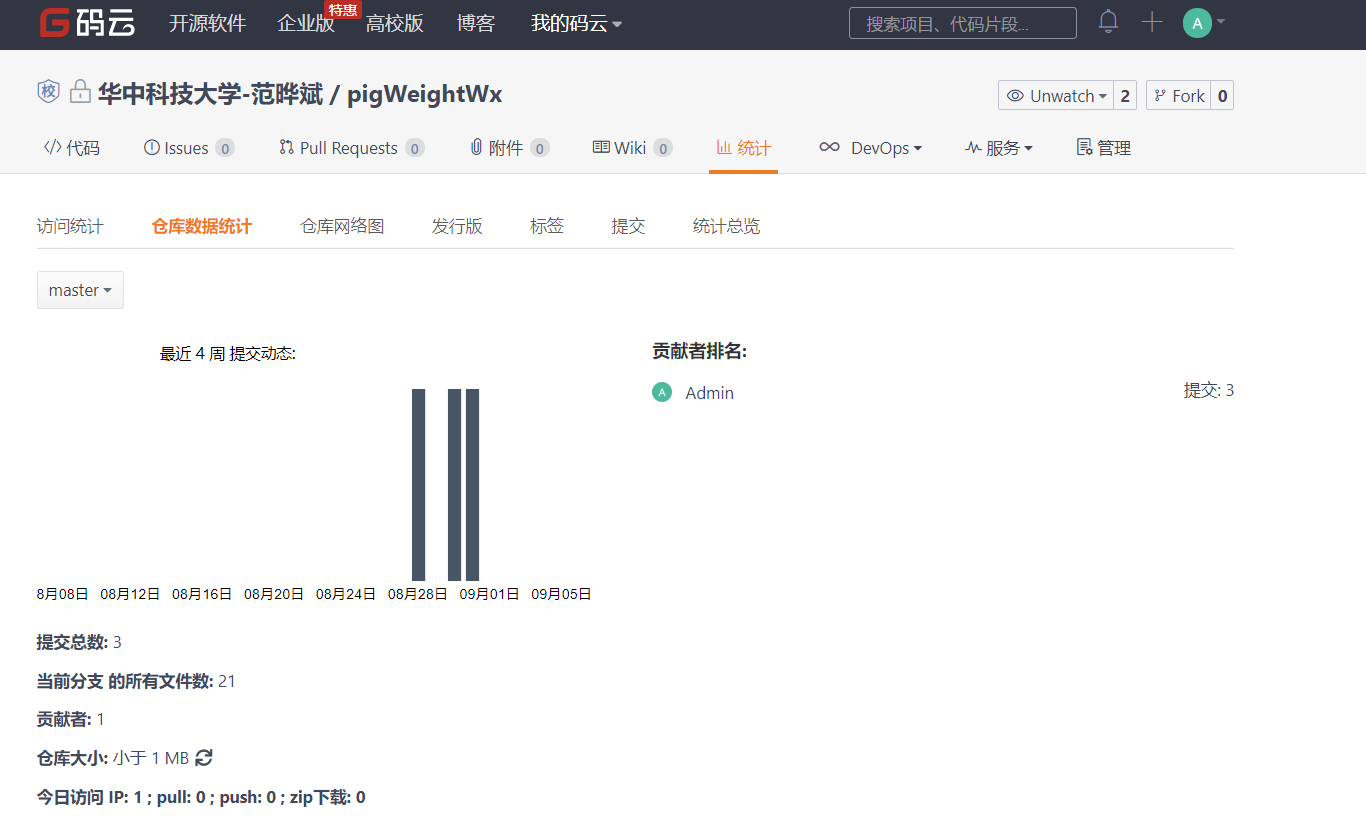
\includegraphics[width=12.4672cm,height=7.657cm]{assets/gitee-example.png}
\end{WordParagraph}

% 原文段落 156；图4-1 码云平台代码签入示例
\begin{WordParagraph}{center}{12}{\WordAutoLine{12}{1}}{0}{0}{24}{0}{0}
\WordAutoSpaceOff
\WordRun{Song}{Song}{12}{0}{0}{000000}{0}{图}%
\WordRun{Times}{Song}{12}{0}{0}{000000}{0}{4-1}%
\WordRun{Song}{Song}{12}{0}{0}{000000}{0}{\WordSpace{1}码云平台代码签入示例}
\end{WordParagraph}

% 原文段落 157；4.2 关键函数说明（黑体4号加粗,字母、阿拉伯数字为Time New Roman4号加粗）
\begin{WordParagraph}{both}{14}{\WordAutoLine{14}{1.25}}{0}{0}{0}{7.8}{7.8}
\WordAutoSpaceOn
\WordRun{Times}{Song}{14}{1}{0}{000000}{0}{4.2}%
\WordRun{Hei}{Hei}{14}{1}{0}{000000}{0}{\WordSpace{1}关键函数说明}%
\WordRun{Kai}{Kai}{12}{0}{0}{FF0000}{0}{（黑体4号加粗,字母、阿拉伯数字为Time\WordSpace{1}New\WordSpace{1}Roman4号加粗）}
\end{WordParagraph}

% 原文段落 158；程序代码部分在这里不需要给出来，只需要叙述清楚在系统中包括哪些函数，各函数的说明，如何利用这些函数实现系统各模块的功能，以及函数间的调用关系（可用图表示出来）。程序详见附录。
\begin{WordParagraph}{both}{12}{\WordAutoLine{12}{1.5}}{0}{0}{24}{0}{0}
\WordAutoSpaceOn
\WordRun{Song}{Song}{12}{0}{0}{000000}{0}{程序代码部分在这里不需要给出来，只需要叙述清楚在系统中包括哪些函数，各函数的说明，如何利用这些函数实现系统各模块的功能，以及函数间的调用关系（可用图表示出来）。程序详见附录。}
\end{WordParagraph}

% 原文段落 159；4.3 测试计划和测试用例（黑体4号加粗,字母、阿拉伯数字为Time New Roman4号加粗）
\begin{WordParagraph}{both}{14}{\WordAutoLine{14}{1.25}}{0}{0}{0}{7.8}{7.8}
\WordAutoSpaceOn
\WordRun{Times}{Song}{14}{1}{0}{000000}{0}{4.3}%
\WordRun{Hei}{Hei}{14}{1}{0}{000000}{0}{\WordSpace{1}测试计划和测试用例}%
\WordRun{Kai}{Kai}{12}{0}{0}{FF0000}{0}{（黑体4号加粗,字母、阿拉伯数字为Time\WordSpace{1}New\WordSpace{1}Roman4号加粗）}
\end{WordParagraph}

% 原文段落 160；首先叙述一下常用的软件测试方法，在选择几个主要的功能模块（自行掌握数量，关键要体现你的水平的一些模块）描述测试过程，（1）先明确模块的功能、设计目标等。（2）分析、叙述如何选取测试数据，要求有完整的测
\begin{WordParagraph}{both}{12}{22.5}{0}{0}{24}{0}{0}
\WordAutoSpaceOff
\WordRun{Song}{Song}{12}{0}{0}{000000}{0}{首先叙述一下常用的软件测试方法，在选择几个主要的功能模块（自行掌握数量，关键要体现你的水平的一些模块）描述测试过程，（1）先明确模块的功能、设计目标等。（2）分析、叙述如何选取测试数据，要求有完整的测试计划和测试用例，说明测试运行结果（这时可用截图）。}
\end{WordParagraph}

% 原文段落 161；4.4 结果分析（黑体4号加粗,字母、阿拉伯数字为Time New Roman4号加粗）
\begin{WordParagraph}{both}{14}{\WordAutoLine{14}{1.25}}{0}{0}{0}{7.8}{7.8}
\WordAutoSpaceOn
\WordRun{Times}{Song}{14}{1}{0}{000000}{0}{4.4}%
\WordRun{Hei}{Hei}{14}{1}{0}{000000}{0}{\WordSpace{1}结果分析}%
\WordRun{Kai}{Kai}{12}{0}{0}{FF0000}{0}{（黑体4号加粗,字母、阿拉伯数字为Time\WordSpace{1}New\WordSpace{1}Roman4号加粗）}
\end{WordParagraph}

% 原文段落 162；根据测试分析运行结果、确认软件是否满足需求。
\begin{WordParagraph}{both}{12}{\WordAutoLine{12}{1.25}}{0}{0}{24}{7.8}{7.8}
\WordAutoSpaceOn
\WordRun{Song}{Song}{12}{0}{0}{000000}{0}{根据测试分析运行结果、确认软件是否满足需求。}
\end{WordParagraph}

% 原文段落 163；
\newpage
\begin{WordParagraph}{left}{12}{\WordAutoLine{12}{1}}{0}{0}{0}{0}{0}
\WordAutoSpaceOn
\WordEmpty
\end{WordParagraph}
